\documentclass[aspectratio=169,11pt]{beamer}
% ==========================================================================
%  KSA lecture-slide theme  =  stock beamer "Boadilla"  +  KSA colour theme
%  brand colours sampled from the official KSA symbol mark:
%    Deep Prussian Blue  #2E3192   (지성 - intellect)
%    Golden Gray         #D6CBB1   (감성 - sensibility)
%  Engine: XeLaTeX.  Usage:
%    \documentclass[aspectratio=169,11pt]{beamer}
%    \input{../../theme/ksa-theme.tex}
%  Each deck lives in its own slides/kor/<deck>/ folder together with its
%  own images; ../../figs/ is kept only as a fallback for the shared cache.
% ==========================================================================

\usepackage{fontspec}
\usepackage{amsmath,amssymb}
\usepackage{graphicx}
\graphicspath{{figs/}{./}{../../../figs/}}
\usepackage{booktabs}
\usepackage{listings}
\usepackage{varwidth}

% ---- fonts (no ctex/xeCJK on this box -> fontspec drives CJK directly) -----
\defaultfontfeatures{Ligatures=TeX}
\setmainfont{Noto Sans CJK KR}
\setsansfont{Noto Sans CJK KR}
\setmonofont{Noto Sans Mono CJK KR}[Scale=0.92]

% ---- base theme: stock Boadilla ------------------------------------------
\usetheme{Boadilla}
\usefonttheme{professionalfonts}
\setbeamertemplate{navigation symbols}{}

% ---- KSA colour theme (recolour the stock theme) --------------------------
\definecolor{ksablue}{HTML}{2E3192}
\definecolor{ksabluedk}{HTML}{20226A}
\definecolor{ksagold}{HTML}{D6CBB1}
\definecolor{ksagolddk}{HTML}{A9976B}
\definecolor{ksared}{HTML}{C0392B}
\definecolor{ksagray}{HTML}{5B5B5B}

\setbeamercolor{structure}{fg=ksablue}
\setbeamercolor{alerted text}{fg=ksared}

\setbeamercolor{palette primary}{fg=white,           bg=ksablue}
\setbeamercolor{palette secondary}{fg=white,         bg=ksablue!85!black}
\setbeamercolor{palette tertiary}{fg=white,          bg=ksabluedk}
\setbeamercolor{titlelike}{fg=ksablue}
\setbeamercolor{frametitle}{fg=ksablue,bg=}
\setbeamercolor{title}{fg=ksablue}
\setbeamercolor{author}{fg=ksagray}
\setbeamercolor{institute}{fg=ksagray}
\setbeamercolor{block title}{fg=white,bg=ksablue}
\setbeamercolor{block body}{fg=black!85,bg=ksablue!6}
\setbeamercolor{item}{fg=ksablue}
\setbeamercolor{section in toc}{fg=black!85}

\setbeamerfont{frametitle}{series=\bfseries}
\setbeamerfont{title}{series=\bfseries}

% ---- footline:  KSA mark | "Made by ..." | n / N   (matches reference) ----
\newcommand{\ksacredit}{}
\setbeamertemplate{footline}{%
  \hbox{%
    \begin{beamercolorbox}[wd=.18\paperwidth,ht=2.6ex,dp=1.5ex,leftskip=1.1em]{}%
      \raisebox{-0.35ex}{\includegraphics[height=2.0ex]{ksa-logo.png}}%
    \end{beamercolorbox}%
    \begin{beamercolorbox}[wd=.64\paperwidth,ht=2.6ex,dp=1.5ex,center]{}%
      {\scriptsize\color{ksagray}\ksacredit}%
    \end{beamercolorbox}%
    \begin{beamercolorbox}[wd=.18\paperwidth,ht=2.6ex,dp=1.5ex,rightskip=1.1em]{}%
      \hfill{\scriptsize\color{ksablue}\insertframenumber\,/\,\inserttotalframenumber}%
    \end{beamercolorbox}%
  }%
  \vskip2pt
}

% ---- section divider: stock \sectionpage, KSA-coloured -------------------
\setbeamertemplate{section page}{%
  \begingroup\centering
    {\color{ksagolddk}\rule{0.16\paperwidth}{1pt}}\par\vskip1.0em
    {\usebeamerfont{title}\color{ksablue}\insertsectionhead\par}\vskip1.0em
    {\color{ksagolddk}\rule{0.16\paperwidth}{1pt}}\par
  \endgroup
}
\AtBeginSection[]{\begin{frame}[plain,noframenumbering]\vfill\sectionpage\vfill\end{frame}}

% ---- code listings ------------------------------------------------------------
\lstdefinestyle{ksa}{%
  basicstyle=\ttfamily\scriptsize,
  keywordstyle=\color{ksablue}\bfseries,
  commentstyle=\color{ksagray}\itshape,
  stringstyle=\color{ksagolddk},
  numberstyle=\tiny\color{ksagray},
  backgroundcolor=\color{ksablue!6},
  frame=leftline, framerule=1.4pt, rulecolor=\color{ksablue},
  xleftmargin=1em, aboveskip=0.8em, belowskip=0.4em,
  showstringspaces=false, breaklines=true, language=Python,
}
\lstset{style=ksa}

% ---- handy macros -----------------------------------------------------------
\newcommand{\kb}[1]{\textbf{\color{ksablue}#1}}   % blue keyword
\newcommand{\kq}[1]{\textbf{\color{ksared}#1}}    % red key-question

\setbeamerfont{title}{series=\bfseries,size=\fontsize{24}{30}\selectfont}
\setbeamerfont{subtitle}{series=\bfseries,size=\fontsize{14}{18}\selectfont}
\setbeamerfont{author}{size=\normalsize}
\setbeamerfont{institute}{size=\small}
\graphicspath{{figs/}{../../../../assets/}}
% 쪽 참조: \markpage{이름} 을 프레임 안에 두고, 다른 곳에서 \pref{이름} 으로 (p.N) 을 부른다 (하단 번호와 같은 번호, 클릭하면 이동)
\makeatletter
\newcommand{\markpage}[1]{\protected@write\@auxout{}{\string\newlabel{#1}{{\the\c@framenumber}{}}}\hypertarget{#1}{}}
\newcommand{\pref}[1]{\hyperlink{#1}{\textcolor{ksagolddk}{(p.\ref{#1})}}}
\makeatother

\renewcommand{\ksacredit}{Machine Learning 1 \,\textperiodcentered\, 나이브 베이즈}
\title{나이브 베이즈}
\subtitle{베이즈 정리로 확률을 뒤집어 분류하기}
\author{Machine Learning 1}
\institute{한국과학영재학교 (KSA)}
\date{}
\begin{document}
\begin{frame}[plain,noframenumbering]\titlepage\end{frame}

% --- 2. 오늘의 질문
\begin{frame}{오늘의 질문}
\vfill
\centering
\includegraphics[width=0.72\linewidth]{nb_mail.png}
\vfill
\note{메일 제목에 무료, 당첨 같은 단어가 들어 있습니다. 이 메일은 스팸일까요? 사람은 감으로 알지만, 컴퓨터는 확률로 판단합니다. 오늘은 그 계산의 핵심인 베이즈 정리와, 이를 이용한 분류기 나이브 베이즈를 배웁니다.}
\end{frame}

% --- 3. 조건부 확률 = 범위를 좁혀서 세기
\begin{frame}{조건부 확률 = 범위를 좁혀서 세기}
\vfill
\centering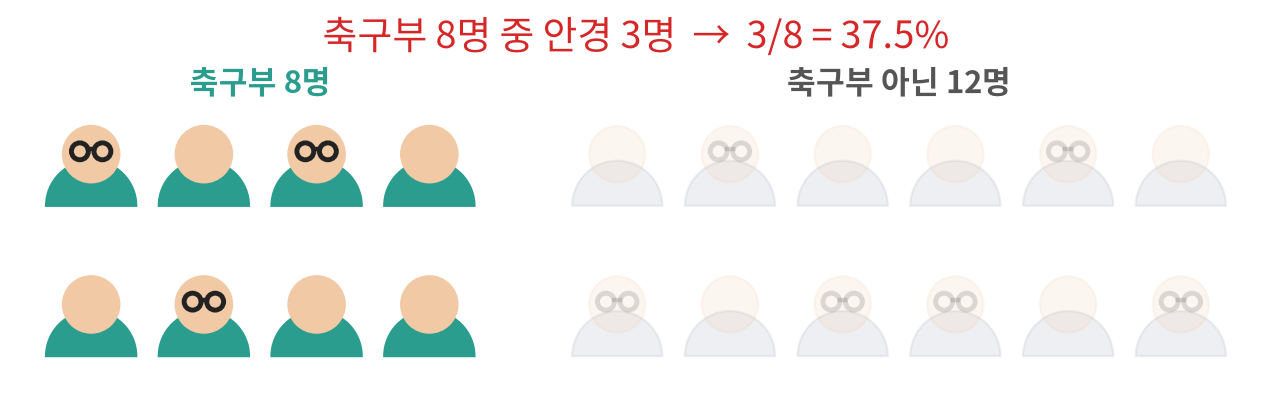
\includegraphics[width=0.8\linewidth]{nb_class_soccer.png}\par\vskip0.4em\LARGE $P(\text{glasses} \mid \text{soccer}) = \dfrac{3}{8}$
\vfill
\note{먼저 조건부 확률부터 보겠습니다. 우리 반 20명 중 축구부가 8명, 안경 쓴 사람이 9명, 둘 다인 사람이 3명입니다. 축구부 중에서 안경 쓴 사람의 비율은? 축구부 8명만 남기고 세면 안경은 3명, 8분의 3입니다. 세로 막대는 '그 사람들 중에서'라는 뜻이고, 조건은 보는 범위를 좁히는 것입니다.}
\end{frame}

% --- 4. 순서를 바꾸면?
\begin{frame}{순서를 바꾸면?}
\vfill
\centering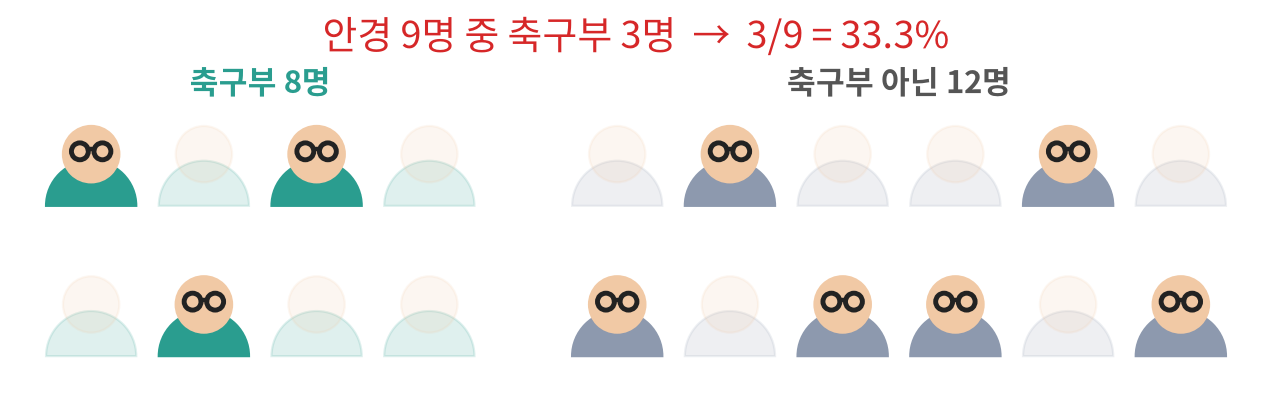
\includegraphics[width=0.8\linewidth]{nb_class_glasses.png}\par\vskip0.4em\LARGE $P(\text{soccer} \mid \text{glasses}) = \dfrac{3}{9} \;\neq\; \dfrac{3}{8}$
\vfill
\note{이번엔 순서를 바꿔 안경 쓴 사람 중 축구부의 비율을 봅시다. 안경 9명만 남기면 축구부는 3명, 9분의 3입니다. 앞의 8분의 3과 다릅니다. 둘 다 '3명'을 세지만, 무엇을 기준으로 나누느냐, 즉 조건이 다르기 때문입니다.}
\end{frame}

% --- 5. 베이즈 정리: 한쪽에서 다른 쪽으로
\begin{frame}{베이즈 정리: 한쪽에서 다른 쪽으로}
\vfill
\centering{\Large\[ P(\text{soccer}\mid\text{glasses}) = \frac{P(\text{glasses}\mid\text{soccer})\;P(\text{soccer})}{P(\text{glasses})} = \frac{\frac{3}{8}\times\frac{8}{20}}{\frac{9}{20}} = \frac{3}{9}\]}\vskip0.6em 직접 센 값과 똑같다
\vfill
\note{베이즈 정리는 한 방향의 조건부 확률에서 반대 방향을 구하는 공식입니다. 8분의 3에 축구부 비율 20분의 8을 곱하면 20분의 3, 즉 둘 다인 사람의 비율이 됩니다. 이것을 안경 비율 20분의 9로 나누면 9분의 3. 직접 센 값과 똑같습니다. 표 전체가 없어도, 이 세 숫자만 알면 반대 방향을 구할 수 있다는 것이 핵심입니다.}
\end{frame}

% --- 6. 아는 것 vs 알고 싶은 것
\begin{frame}{아는 것 vs 알고 싶은 것}
\vfill
\centering\Large 데이터로 셀 수 있는 것: \; $P(\text{`free'} \mid \text{spam})$\\[1.2em] 우리가 알고 싶은 것: \; $P(\text{spam} \mid \text{`free'})$\\[1.2em]\normalsize\kq{방향이 반대다}\\[0.8em]{\footnotesize 수식에서는 `무료'를 `free', 스팸을 spam, 정상을 ham 으로 쓴다}
\vfill
\note{스팸 메일 뭉치를 모아 두면, 스팸에 무료가 몇 번 나오는지는 셀 수 있습니다. 하지만 우리가 알고 싶은 건 반대 방향, 무료가 나온 메일이 스팸일 확률입니다. 이 둘은 같은 값이 아닙니다. 방향을 뒤집는 도구가 베이즈 정리입니다.}
\end{frame}

% --- 7. 베이즈 정리
\begin{frame}{베이즈 정리}
\vfill
\centering{\LARGE\[ \underbrace{P(y\mid x)}_{\text{posterior}} = \frac{\overbrace{P(x\mid y)}^{\text{likelihood}}\;\overbrace{P(y)}^{\text{prior}}}{\underbrace{P(x)}_{\text{evidence}}}\]}
\vfill
\note{일반적인 모양으로 쓰면 이렇습니다. 사후확률은 가능도 곱하기 사전확률, 나누기 증거입니다. 사전확률은 아무것도 보기 전에 스팸이 얼마나 흔한지, 가능도는 스팸이라면 이 단어가 나올 확률, 증거는 이 단어가 나올 전체 확률입니다.}
\end{frame}

% --- 7b. 베이즈 정리: 용어 (한글)
\begin{frame}{베이즈 정리: 용어 (한글)}
\vfill
\centering{\LARGE\[ \underbrace{P(y\mid x)}_{\text{사후확률}} = \frac{\overbrace{P(x\mid y)}^{\text{가능도}}\;\overbrace{P(y)}^{\text{사전확률}}}{\underbrace{P(x)}_{\text{증거}}}\]}
\vskip0.4em
\renewcommand{\arraystretch}{1.3}
{\normalsize\begin{tabular}{rll}
\kb{사후확률} & posterior & 증거 $x$를 본 뒤에 $y$일 확률\\
\kb{가능도} & likelihood & $y$라면 $x$가 나올 확률\\
\kb{사전확률} & prior & 아무것도 보기 전에 $y$일 확률\\
\kb{증거} & evidence & $x$가 나올 전체 확률 (스팸이든 정상이든)
\end{tabular}}
\vfill
\note{앞 쪽의 영어 이름을 우리말로 옮기면 이렇습니다. posterior는 사후확률, 증거를 본 뒤에 y일 확률입니다. likelihood는 가능도, y라면 x가 나올 확률입니다. prior는 사전확률, 아무것도 보기 전에 y일 확률입니다. evidence는 증거, x가 나올 전체 확률입니다.}
\end{frame}

% --- 8. 1000통으로 세어 보기
\begin{frame}{1000통으로 세어 보기}
\vfill
\centering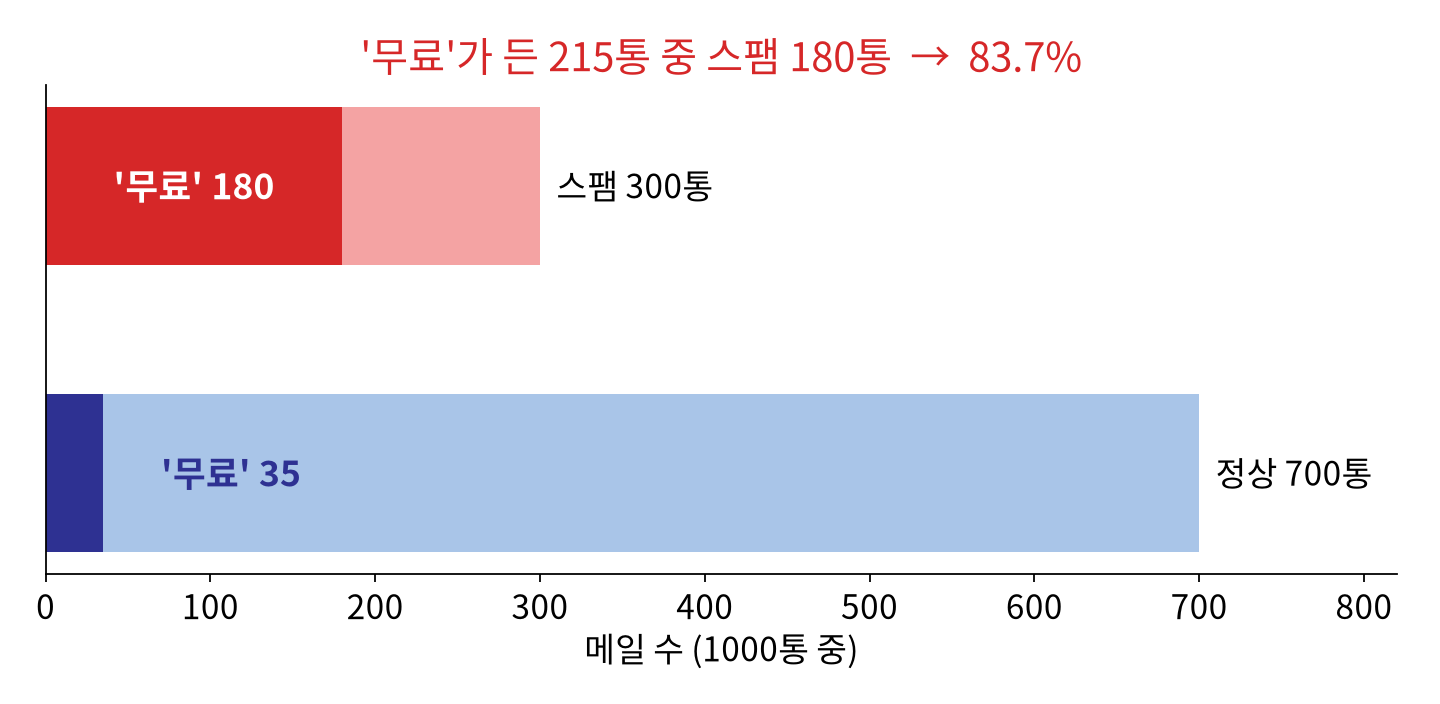
\includegraphics[width=0.78\linewidth]{nb_tree.png}
\vfill
\note{숫자로 세어 봅시다. 메일의 30퍼센트가 스팸이고, 무료는 스팸의 60퍼센트, 정상 메일의 5퍼센트에 나온다고 합시다. 1000통이면 스팸 300통 중 180통, 정상 700통 중 35통에 무료가 있습니다. 무료가 든 215통 중 스팸은 180통, 약 83.7퍼센트입니다. 베이즈 정리는 이 세기를 식으로 쓴 것뿐입니다.}
\end{frame}

% --- 9. 증거가 쌓이면
\begin{frame}{증거가 쌓이면}
\vfill
\begin{columns}[c]
  \begin{column}{0.56\textwidth}
    \centering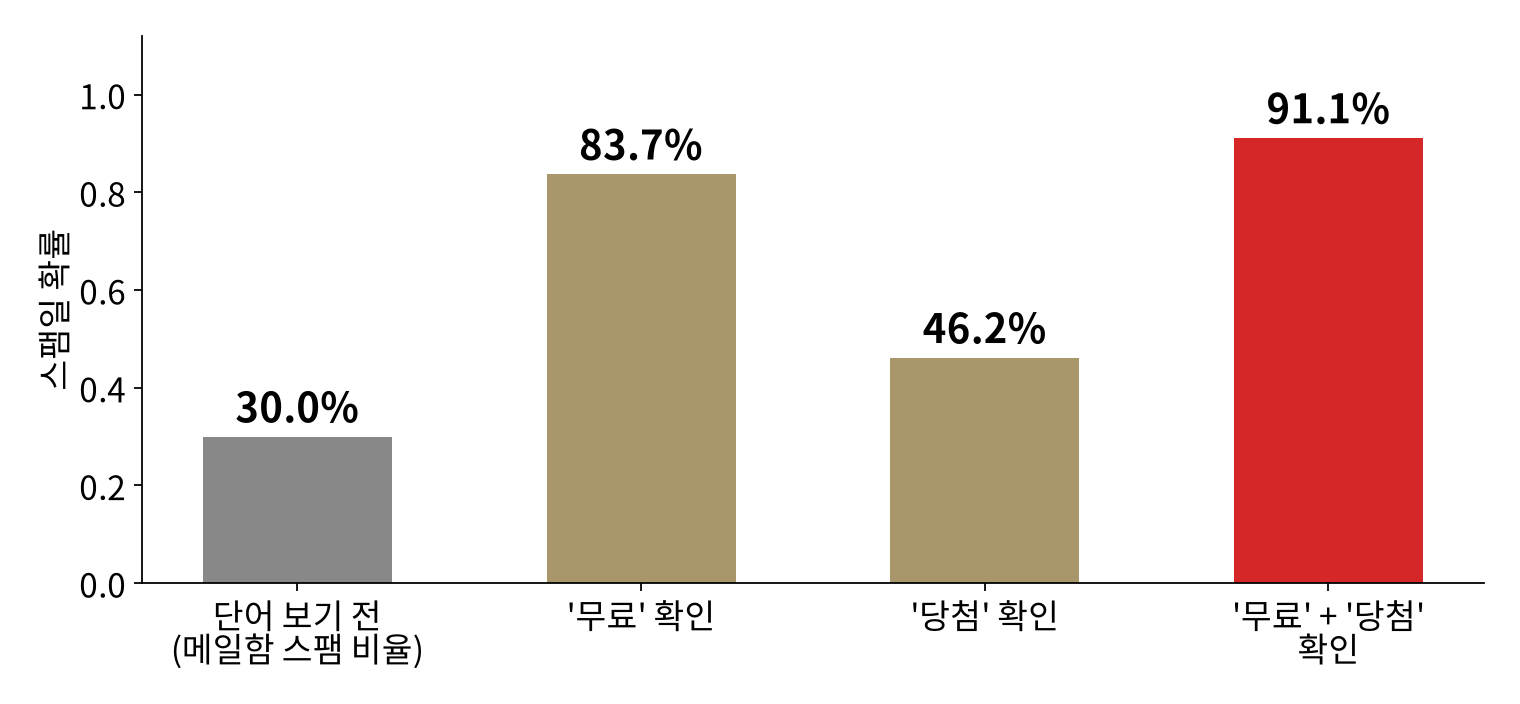
\includegraphics[width=\linewidth]{nb_update.png}
  \end{column}
  \begin{column}{0.42\textwidth}
    \centering
    {\small 1000통에서 단어가 든 메일만 남기며 센다}\\[0.4em]
    \renewcommand{\arraystretch}{1.35}
    {\small\setlength{\tabcolsep}{4pt}\begin{tabular}{l|rr|r}
     & 스팸 & 정상 & 스팸 비율\\\hline
    처음 & 300 & 700 & 30\%\\
    `무료' & 180 & 35 & 83.7\%\\
    `당첨' & 120 & 140 & 46.2\%\\
    `무료'+`당첨' & 72 & 7 & \kq{91.1\%}
    \end{tabular}}\\[0.6em]
    {\footnotesize 곱하는 비율 (스팸 / 정상)\\ `무료' 0.6 / 0.05 \quad `당첨' 0.4 / 0.2}
  \end{column}
\end{columns}
\vfill
\note{단어를 보기 전에는 메일함의 스팸 비율 그대로 30퍼센트입니다. 무료만 보면 83.7퍼센트, 당첨만 보면 46.2퍼센트이고, 두 단어를 모두 보면 91.1퍼센트가 됩니다. 당첨은 무료보다 약한 증거라서 혼자서는 확률이 덜 오르지만, 둘이 함께 나오면 더 올라갑니다. 앞 단계의 사후확률이 다음 단계의 사전확률이 되어, 증거가 쌓일수록 확신이 커집니다. 주의할 점은 83.7과 89.6을 곱하는 게 아니라는 것입니다. 곱하면 0.75밖에 안 됩니다. 1000통으로 세어 봅시다. 처음에 스팸 300통, 정상 700통입니다. 무료가 든 메일만 남기면 스팸은 180통, 정상은 35통입니다. 당첨만 남기면 스팸은 120통, 정상은 140통입니다. 두 단어가 모두 든 메일만 남기면 스팸은 72통, 정상은 7통이 남습니다. 스팸 비율은 72를 79로 나눈 91.1퍼센트입니다. 단어를 볼 때마다 정상이 스팸보다 더 많이 줄어드는 구조가 나이브 베이즈입니다.}
\end{frame}

% --- 10. 스팸이 드문 메일함이라면?
\begin{frame}{스팸이 드문 메일함이라면?}
\vfill
\centering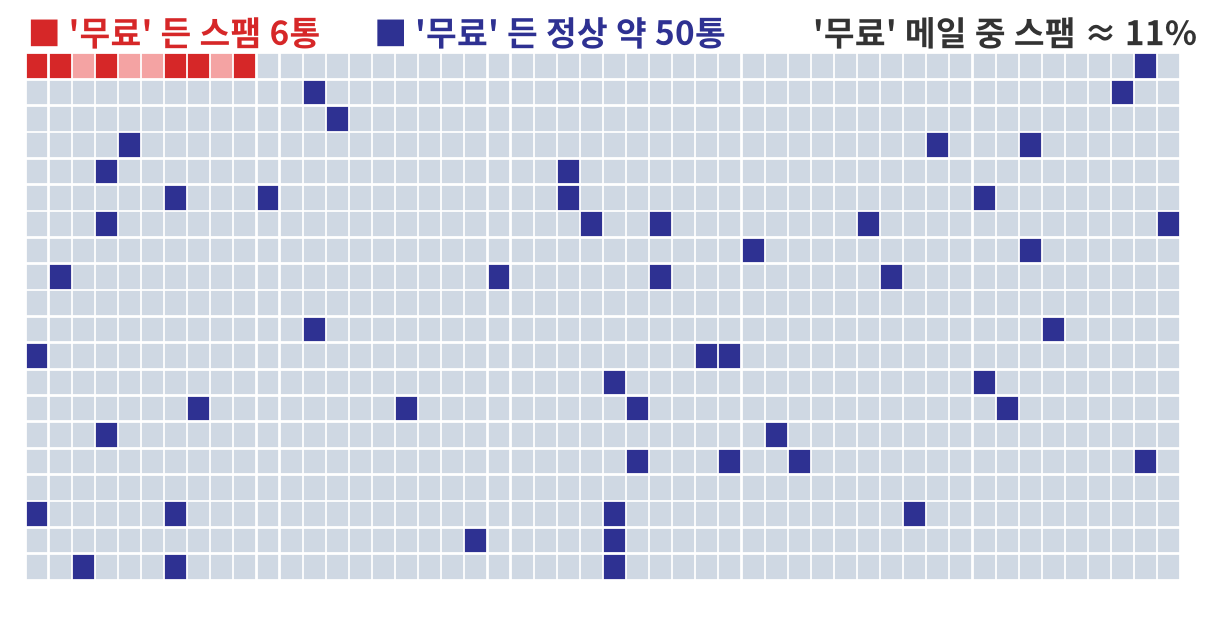
\includegraphics[width=0.78\linewidth]{nb_grid.png}\par\vskip0.3em 스팸이 1\%뿐인 메일함, 같은 `무료'
\vfill
\note{이번엔 회사 메일함처럼 스팸이 1퍼센트뿐인 곳을 생각해 봅시다. 단어 확률은 똑같이 스팸의 60퍼센트, 정상의 5퍼센트에 무료가 나옵니다. 1000통 중 스팸은 10통, 그중 무료는 6통. 정상 990통 중 무료는 약 50통입니다. 무료가 든 56통 중 스팸은 6통, 약 11퍼센트에 불과합니다. 같은 단어인데 84퍼센트가 11퍼센트로 떨어졌습니다.}
\end{frame}

% --- 11. 사전확률의 힘
\begin{frame}{사전확률의 힘}
\vfill
\centering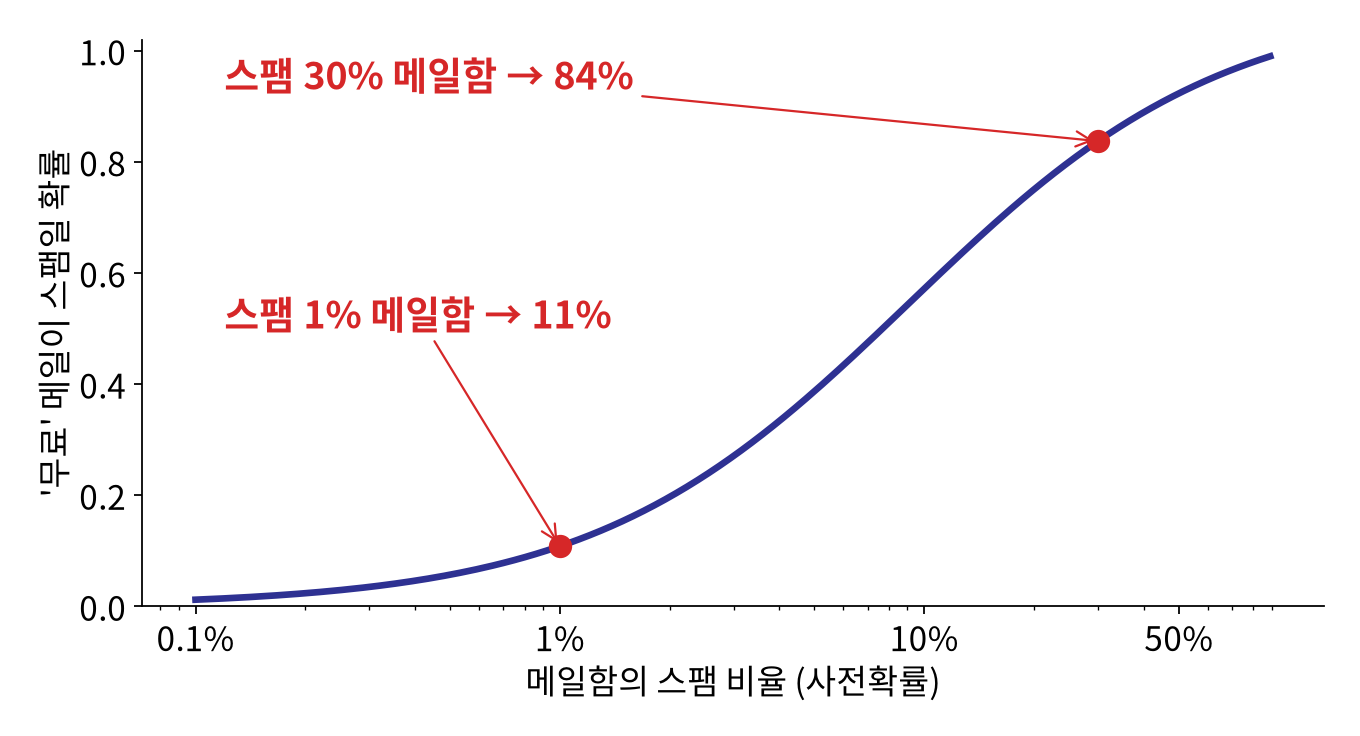
\includegraphics[width=0.72\linewidth]{nb_prior_curve.png}\par\vskip0.3em
{\small 같은 `무료'를 봐도 스팸이 드문 메일함(1\%)이면 \kq{11\%}, 흔한 메일함(30\%)이면 \kq{84\%} \\ $\rightarrow$ 결론은 \kb{처음 비율(사전확률)}에 따라 달라진다}
\vfill
\note{증거가 같아도 사전확률, 즉 원래 스팸이 얼마나 흔한지에 따라 결론이 완전히 달라집니다. 스팸이 30퍼센트인 메일함에선 84퍼센트, 1퍼센트인 메일함에선 11퍼센트입니다. 사전확률을 무시하고 단어만 보면 크게 틀리는데, 이것을 기저율 오류라고 합니다. 계산은 다음 쪽에서 봅니다.}
\end{frame}

% --- 11b. 사전확률의 힘: 30%
\begin{frame}{사전확률의 힘: 스팸 30\% 메일함}
\vfill
\centering
{\Large\[ \underbrace{P(\text{spam}\mid\text{`free'})}_{\text{posterior}} = \frac{{\color{ksablue}0.60}\times{\color{ksared}0.30}}{\underbrace{{\color{ksablue}0.60}\times{\color{ksared}0.30}+{\color{ksablue}0.05}\times{\color{ksared}0.70}}_{\text{evidence}}} \approx \kq{84\%}\]}
\vskip0.3em
\renewcommand{\arraystretch}{1.3}
{\normalsize\begin{tabular}{rl}
{\color{ksablue}\textbf{0.60, 0.05}} & \textbf{likelihood (가능도)}: $P(\text{`free'}\mid\text{spam})$, $P(\text{`free'}\mid\text{ham})$\\
{\color{ksared}\textbf{0.30, 0.70}} & \textbf{prior (사전확률)}: $P(\text{spam})$, $P(\text{ham})=1-P(\text{spam})$\\
\textbf{분모 전체} & \textbf{evidence (증거)}: $P(\text{`free'})$ = `무료'가 든 모든 메일\\
\textbf{84\%} & \textbf{posterior (사후확률)}: 구하려는 값
\end{tabular}}
\vfill
\note{식의 각 숫자가 무엇인지 봅시다. 파란색 0.60과 0.05는 가능도입니다. 스팸에서 무료가 나올 확률 0.60, 정상에서 무료가 나올 확률 0.05입니다. 빨간색 0.30과 0.70은 사전확률입니다. 스팸일 확률 0.30, 정상일 확률은 1에서 0.30을 뺀 0.70입니다. 분모 전체는 증거, 즉 무료가 든 모든 메일의 비율이고, 분자는 스팸이면서 무료가 든 메일의 비율입니다. 구하려는 값인 사후확률은 0.18을 0.215로 나눈 약 84퍼센트입니다. 0.60은 사후확률이 아니라 가능도입니다.}
\end{frame}

% --- 11c. 사전확률의 힘: 1%
\begin{frame}{사전확률의 힘: 스팸 1\% 메일함}
\vfill
\centering
{\Large\[ \underbrace{P(\text{spam}\mid\text{`free'})}_{\text{posterior}} = \frac{{\color{ksablue}0.60}\times{\color{ksared}0.01}}{\underbrace{{\color{ksablue}0.60}\times{\color{ksared}0.01}+{\color{ksablue}0.05}\times{\color{ksared}0.99}}_{\text{evidence}}} \approx \kq{11\%}\]}
\vskip0.3em
\renewcommand{\arraystretch}{1.3}
{\normalsize\begin{tabular}{rl}
{\color{ksablue}\textbf{0.60, 0.05}} & \textbf{likelihood (가능도)}: $P(\text{`free'}\mid\text{spam})$, $P(\text{`free'}\mid\text{ham})$\\
{\color{ksared}\textbf{0.01, 0.99}} & \textbf{prior (사전확률)}: $P(\text{spam})$, $P(\text{ham})=1-P(\text{spam})$\\
\textbf{분모 전체} & \textbf{evidence (증거)}: $P(\text{`free'})$ = `무료'가 든 모든 메일\\
\textbf{11\%} & \textbf{posterior (사후확률)}: 구하려는 값
\end{tabular}}
\vfill
\note{같은 식에서 사전확률만 바꿨습니다. 가능도 0.60과 0.05는 그대로이고, 사전확률이 스팸 0.01, 정상 0.99로 바뀝니다. 분자는 0.60 곱하기 0.01로 0.006, 분모는 0.006 더하기 0.05 곱하기 0.99로 0.0555입니다. 사후확률은 약 11퍼센트입니다. 같은 단어를 봐도 사전확률이 작으면 사후확률이 크게 떨어집니다.}
\end{frame}

% --- 12. 분류 규칙
\begin{frame}{분류 규칙}
\vfill
\centering{\LARGE\[ \hat y = \arg\max_{y}\; P(y)\,P(x\mid y)\]}\vskip0.6em 분모 $P(x)$는 모든 $y$에 같으니 비교할 땐 빼도 된다
\vfill
\note{분류할 때는 스팸과 정상 중 사후확률이 큰 쪽을 고르면 됩니다. 분모의 증거는 두 클래스에 똑같으니, 사전확률 곱하기 가능도만 비교하면 됩니다.}
\end{frame}

% --- 13. 문제: 단어가 많으면?
\begin{frame}{문제: 단어가 많으면?}
\vfill
\centering{\LARGE\[ P(x_1, x_2, \dots, x_n \mid y)\]}\vskip0.6em $x_i$: 단어 $i$가 메일에 있으면 1, 없으면 0\\[0.4em] 단어 1만 개 $\Rightarrow$ 가능한 조합 $2^{10000}$개
\vfill
\note{그런데 메일에는 단어가 여러 개입니다. 단어마다 메일에 있다, 없다 두 경우가 있으니, 단어가 만 개이면 조합이 2의 만 제곱 개나 됩니다. 이 모든 조합을 데이터로 셀 수는 없습니다.}
\end{frame}

% --- 13b. 정확한 식: 연쇄 법칙
\begin{frame}{정확한 식: 연쇄 법칙}
\vfill
\centering
{\small 단어 두 개}\\[0.3em]
{\Large $P(x_1,x_2\mid y) = P(x_2\mid x_1,y)\;P(x_1\mid y)$}\\[1.4em]
{\small 단어 $n$개}
\[ P(x_1,\dots,x_n\mid y) = P(x_1\mid y)\,P(x_2\mid x_1,y)\,P(x_3\mid x_1,x_2,y)\cdots P(x_n\mid x_1,\dots,x_{n-1},y) \]
\kq{항상 성립하는 식} \quad 뒤로 갈수록 조건이 늘어난다 $\Rightarrow$ 데이터로 세기 어렵다
\vfill
\note{단어 조합의 확률은 사실 이렇게 쓸 수 있습니다. 확률의 연쇄 법칙이라고 하는데, 가정이 아니라 항상 성립하는 식입니다. 단어가 두 개면, 첫 단어의 확률에 첫 단어가 나왔을 때 둘째 단어가 나올 확률을 곱합니다. 단어가 n개면 단어마다 앞의 모든 단어를 조건으로 가진 확률이 곱해집니다. 문제는 뒤로 갈수록 조건이 늘어난다는 점입니다. 앞 단어들이 모두 이렇게 나온 메일은 데이터에 거의 없어서 세기 어렵습니다.}
\end{frame}

% --- 14. 나이브 가정: 단어끼리 독립
\begin{frame}{나이브 가정: 단어끼리 독립}
\markpage{naiveassump}
\vfill
\centering{\LARGE\[ P(x_1,\dots,x_n\mid y) \approx \prod_{i=1}^{n} P(x_i\mid y)\]}\vskip0.3em {\normalsize $P(x_i\mid x_1,\dots,x_{i-1},y) \;\to\; P(x_i\mid y)$ \quad 앞 단어들을 조건에서 \kq{지운다}}\vskip0.4em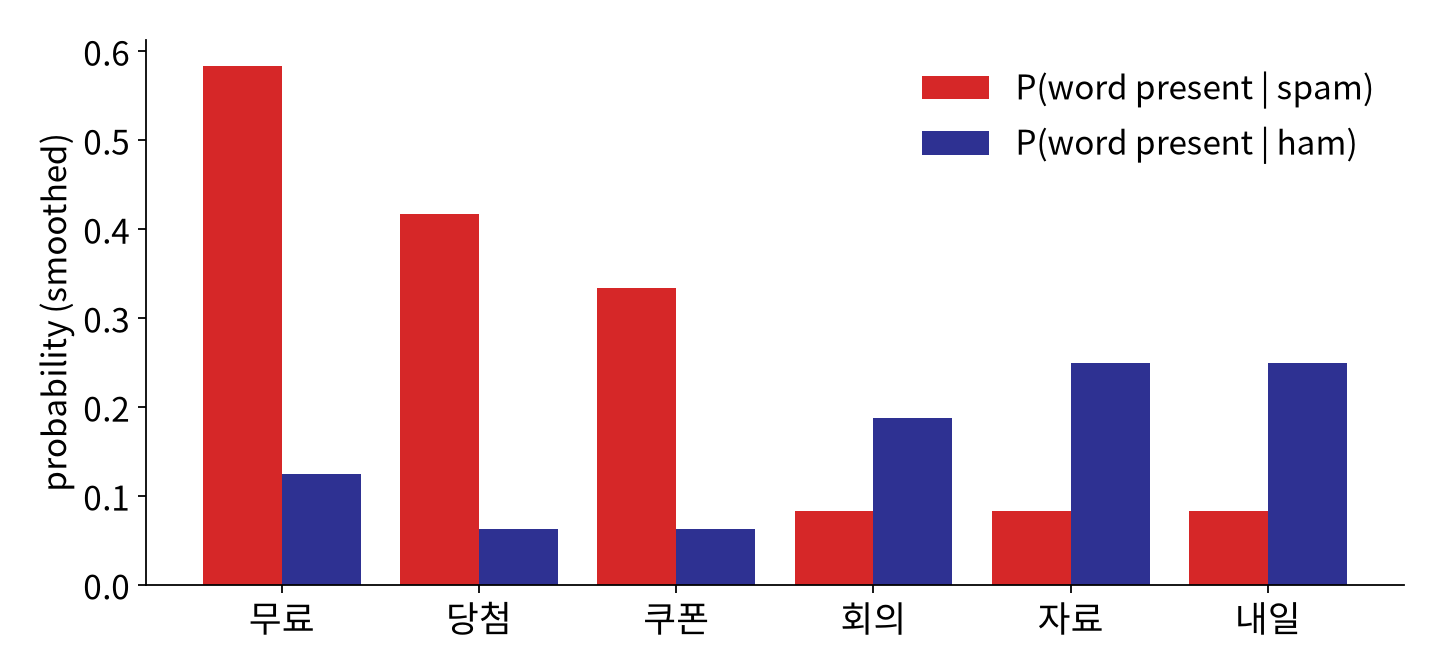
\includegraphics[width=0.46\linewidth]{nb_words.png}
\vfill
\note{그래서 과감하게 가정합니다. 클래스를 알면 단어들은 서로 독립이다. 앞 단어들을 조건에서 지우는 겁니다. 그러면 조합 확률이 단어별 확률의 곱이 되고, 단어마다 스팸 메일과 정상 메일에서 그 단어가 있을 확률만 세면 됩니다. 단어가 없을 확률은 1에서 빼면 됩니다. 현실과 다른 순진한 가정이라 나이브라는 이름이 붙었지만, 스팸 분류에서는 놀랍게 잘 작동합니다.}
\end{frame}

% --- 15. 0 하나가 전부를 지운다
\begin{frame}{0 하나가 전부를 지운다}
\vfill
\centering
`내일 회의 \kq{당첨}' \quad (정상 메일인데 `당첨'이 우연히 들어갔다)\vskip0.8em
\renewcommand{\arraystretch}{1.5}
\begin{tabular}{c|cc}
 & $P(\text{present}\mid\text{ham})$ & $P(\text{present}\mid\text{spam})$\\\hline
내일 & $3/14$ & \textcolor{ksared}{$0/10$}\\
회의 & $2/14$ & \textcolor{ksared}{$0/10$}\\
당첨 & \textcolor{ksared}{$0/14$} & $4/10$\\\hline
곱 & \textcolor{ksared}{\textbf{0}} & \textcolor{ksared}{\textbf{0}}
\end{tabular}\vskip0.6em
\kq{둘 다 0 $\Rightarrow$ 어느 쪽인지 판단할 수 없다}\\[0.4em]
{\footnotesize 정상 14통, 스팸 10통 기준. 없는 단어는 $1-P$를 곱하지만 여기서는 생략}
\vfill
\note{학습 데이터에서 한 번도 못 본 단어가 있으면 그 단어의 확률은 0입니다. 그리고 확률을 곱하는 순간 전체가 0이 됩니다. 정상 메일 14통 중 당첨이 든 메일이 한 통도 없었으니 정상 쪽이 0이고, 스팸 메일 10통에는 내일과 회의가 든 메일이 한 통도 없었으니 스팸 쪽도 0입니다. 두 점수가 모두 0이라 어느 쪽이 더 그럴듯한지 비교할 수 없습니다. 단어 하나 때문에 판단이 망가지는 거죠.}
\end{frame}

% --- 16. 해결: 가상 메일을 1통씩 더한다 (라플라스 스무딩)
\begin{frame}{해결: 가상 메일을 1통씩 더한다}
\vfill
\centering
{\LARGE\[ P(x_i=1\mid y) = \frac{n_{i,y} + 1}{M_y + 2}\]}
\renewcommand{\arraystretch}{1.2}
\begin{tabular}{c|cc}
 & $P(\text{present}\mid\text{ham})$ & $P(\text{present}\mid\text{spam})$\\\hline
내일 & $4/16$ & $1/12$\\
회의 & $3/16$ & $1/12$\\
당첨 & \kb{$1/16$} & $5/12$
\end{tabular}\vskip0.4em
정상 \textbf{58.6\%} \quad 스팸 41.4\% \quad $\Rightarrow$ \kb{정상으로 분류} \;{\footnotesize (세 단어만 계산)}\\[0.4em]
{\small $n_{i,y}$: 단어 $i$가 든 $y$ 메일 수 \quad $M_y$: $y$ 메일 수 (정상 14, 스팸 10)\\ \textbf{+2}: `있다'와 `없다' 두 경우에 가상 메일 1통씩}
\vfill
\note{해결책은 간단합니다. 있는 경우와 없는 경우에 가상의 메일을 한 통씩 더합니다. 정상 메일에서 당첨이 든 메일은 0통이었지만 0 더하기 1을 해서 1이 되고, 분모는 메일 수 14에 가상 메일 2통을 더한 16입니다. 분모가 2 늘어나는 이유는 있는 쪽과 없는 쪽에 한 통씩 더했기 때문입니다. 그래야 있을 확률과 없을 확률을 더해서 1이 됩니다. 이제 정상 메일 쪽 점수가 0이 아니어서, 계산하면 정상 58.6퍼센트로 올바르게 분류됩니다.}
\end{frame}

% --- 17. 유도: 로그 사후확률
\begin{frame}{유도: 로그 사후확률}
\vfill
\small
\begin{align*}
\log P(y\mid x_1,\dots,x_n) &= \log \frac{P(x_1,\dots,x_n\mid y)\,P(y)}{P(x_1,\dots,x_n)} && \text{Bayes}\\[0.3em]
&= \log P(x_1,\dots,x_n\mid y) + \log P(y) - \log P(x_1,\dots,x_n) && \text{log}\\[0.3em]
&\approx \sum_{i=1}^{n} \log P(x_i\mid y) + \log P(y) - \log P(x_1,\dots,x_n) && \text{naive \pref{naiveassump}}\\[0.3em]
&= \log P(y) + \sum_{i=1}^{n} \log P(x_i\mid y) + C
\end{align*}
\vskip0.3em
\centering $C=-\log P(x_1,\dots,x_n)$ 은 $y$와 무관한 상수 $\Rightarrow$ \kb{비교할 땐 빼도 된다}
\vfill
\note{베이즈 정리에서 시작해서 로그를 씌워 봅시다. 먼저 베이즈 정리로 사후확률을 가능도 곱하기 사전확률, 나누기 증거로 씁니다. 여기에 로그를 취하면 곱은 합이 되고 나눗셈은 뺄셈이 됩니다. 다음으로 나이브 가정, 즉 단어끼리 독립이라는 가정을 쓰면 가능도의 로그가 단어별 로그의 합이 됩니다. 마지막 항, 증거에 로그를 취한 값은 스팸이든 정상이든 똑같은 상수이므로 C라고 두고, 클래스를 비교할 때는 빼도 됩니다. 현실의 단어들은 완전히 독립이 아니라서, 이 줄은 같다가 아니라 거의 같다로 씁니다. 앞에서 본 나이브 가정 쪽의 식과 같은 기호입니다.}
\end{frame}

% --- 18. 곱 대신 로그의 합
\begin{frame}{곱 대신 로그의 합}
\vfill
\centering\makebox[\linewidth][c]{\fontsize{19}{24}\selectfont$\displaystyle \log P(y\mid x_1,\dots,x_n) \,\propto\, \log P(y) + \sum_{i=1}^{n} \log P(x_i\mid y)$}\vskip0.6em 작은 확률을 수백 번 곱하면 컴퓨터에선 0이 된다\\[0.3em]{\small (0.01을 200번 곱하면 $10^{-400}$ $\Rightarrow$ 로그를 취해 합으로 계산한다)}
\vfill
\note{이제 결과를 크게 봅시다. 사후확률의 로그는 사전확률의 로그에, 단어별 가능도의 로그를 모두 더한 것에 비례합니다. 곱 대신 로그의 합을 쓰는 이유는, 0.01 같은 작은 확률을 수백 번 곱하면 컴퓨터가 표현할 수 있는 가장 작은 수보다 작아져 0이 되기 때문입니다. 0.01을 200번만 곱해도 10의 마이너스 400제곱입니다. 로그는 큰 수일수록 큰 값이라서, 어느 클래스 점수가 큰지 비교한 결과는 바뀌지 않습니다. 단어가 있으면 있을 확률의 로그를, 없으면 없을 확률의 로그를 더하면 됩니다.}
\end{frame}

% --- 19. 문제풀이
\begin{frame}{문제풀이}
\vfill
\begin{enumerate}\item 메일의 20\%가 스팸이다. `할인'은 스팸의 50\%, 정상의 10\%에 나온다. `할인'이 든 메일이 스팸일 확률은?\vskip1em\item 정상 메일 14통 중 `당첨'(win)이 든 메일이 0통이다. 라플라스 스무딩 후 $P(\text{win}\mid\text{ham})$은?\end{enumerate}
\vfill
\note{문제 두 개를 풀어 봅시다. 1번 답. 분자는 0.2 곱하기 0.5, 0.1이고, 분모는 0.1 더하기 0.8 곱하기 0.1, 0.18입니다. 따라서 약 55.6퍼센트. 2번 답. 0 더하기 1을, 14 더하기 2, 즉 16으로 나눠 1/16, 약 0.0625입니다. 0이 아니게 되었다는 점이 핵심입니다.}
\end{frame}

% --- 20. 실습
\begin{frame}{실습}
\vfill
\centering\begin{tabular}{rl}\large 1 & 베이즈 정리로 `free' 메시지가 스팸일 확률 · 직접 세기 · 사전확률 바꿔 보기\\[0.5em]\large 2 & 나이브 베이즈 직접 구현 (스무딩 · 로그 합) 후 테스트 정확도\\[0.5em]\large 3 & scikit-learn BernoulliNB와 비교\end{tabular}\vskip1em 영어 문자메시지 5,574건 (UCI SMS Spam Collection)\\[0.4em]\textcolor{ksagolddk}{▶ Colab: 실습 노트북}
\vfill
\note{실습은 세 부분입니다. 첫째, 진짜 영어 스팸 문자 데이터에서 free가 든 메시지가 스팸일 확률을 베이즈 정리로 구하고, 직접 세어 본 값과 같은지 확인합니다. 둘째, 나이브 베이즈를 직접 구현합니다. 스무딩과 로그 합 부분을 채우면 됩니다. 셋째, scikit-learn의 BernoulliNB 결과와 같은지 비교합니다.}
\end{frame}

% --- 21. 정리
\begin{frame}{정리}
\vfill
\centering\large\begin{tabular}{l}베이즈 정리 \quad 사후 $\propto$ 가능도 $\times$ 사전\\[0.5em]사전확률 \quad 원래 얼마나 흔한가가 결론을 바꾼다\\[0.5em]나이브 가정 \quad 단어별 확률의 곱\\[0.5em]실전 \quad 라플라스 스무딩 + 로그 합\end{tabular}
\vfill
\note{정리합니다. 베이즈 정리는 확률의 방향을 뒤집는 도구이고, 사후확률은 가능도와 사전확률의 곱에 비례합니다. 같은 단어라도 스팸이 얼마나 흔한지, 즉 사전확률에 따라 결론이 달라집니다. 나이브 베이즈는 단어끼리 독립이라 가정해 확률을 곱하고, 실전에서는 라플라스 스무딩과 로그 합을 씁니다.}
\end{frame}
\end{document}
